
\section{Seismicity of Northern Iran}

We are interested in applying the visibility graph method to northern Iran. This region is part of the Iranian plateau, on the Himalayan-Alpine seismic belt. It is confined by the relative movements between the Arabian, Eurasian, eastern Asia-Minor, and Indian plates; and has a long history of large magnitude ($M>7$) earthquakes that are well documented dating back to the eight century \citep[e.g.,][]{Berberian_1981_Chap}. According to the tectonic settings and geologic provinces of the plateau, the seismic activity in Iran has been categorized into different seismic zones. These vary between four to nine major seismic zones, in the more traditional models \citep[e.g.,][]{Stocklin1968, Takin1972, Berberian1976}, up to twenty to twenty-three seismotectonic provinces in the most elaborate ones \citep[e.g.,][]{Nowroozi1976, Tavakoli1999}. We adopt the model proposed by \citet{Mirzaei1998} with modifications introduced by \citet{Karimiparidari2013}. In it, Iran is divided into six seismic regions: Azerbaijan, Alborz, Kopeh-Dagh, Zagros, Central-East Iran, and Makran. Our focus, however, is on the northern part of Iran, for which we define a region of interest between longitudes 43.5\textdegree{}E and 61.5\textdegree{}E, and latitudes 34\textdegree{}N and 40\textdegree{}N, as shown in Fig.~\ref{fig:study_region}. Although this region encloses part of the Zagros and Central-East seismic zones, we concentrate in the analysis of the seismicity of Azerbaijan, Alborz and Kopeh-Dagh.

\begin{figure*}[t]
	\centering
	\includegraphics[width=\textwidth]{figures/pdf/figure-02} 
	\caption{Region of interest, highlighting the seismic zones that are the focus of this study (Azerbaijan, Alborz, and Kopeh-Dagh) for the application of the visibility graph method. The top-right location map shows Iran and the selected area with respect to neighboring countries. The solid dark lines show the boundaries of the additional Zagros and Central-East seismic zones. This zonation follows the divisinos proposed and madofied by \citet{Mirzaei1998} and \citet{Karimiparidari2013}, respectively.}
	\label{fig:study_region}
\end{figure*}

Northern Iran houses about 41 percent (32 million) of the total population of the country, and has suffered devastating earthquakes in the past \citep[e.g.,][]{Mehrain_1990_Tech, Chafory-Ashtiany_1999_DPM, Razzaghi_2012_Tech}. At the northwest, the seismic zone of Azerbaijan is strongly controlled by the North Tabriz Fault system in the vicinity of the city of Tabriz, shown in Fig.~\ref{fig:study_region}. Historical accounts document the occurrence of strong $M>6$ earthquakes in this region as far back as the ninth century \citep{Berberian1999}, and a few $M>7$ earthquakes in 1042, 1721 and 1780 \citep{Jones1834}. More recently, this region was struck by the $M_w$ 6.1 1997 Ardabil earthquake near the city of Ardabil and $M_w$ 6.4 2012 Tabriz earthquake northeast of the city of Tabriz. These earthquakes caused extensive damage and took the lives of more than 1500 people. 

The seismicity in the north-central region of Alborz is dominated by multiple fault systems, including the Talesh, Rubdar, North Alborz, and North Tehran faults, which also have a history of producing strong ground shaking. According to \citet{Ambraseys_1982_Book}, Tehran was devastated by severe $M>7$ earthquakes in 743, 958, 1177, 1665, and 1830. This region has also seen some significant recent seismic activity \citep{Berberian1999}, including the $M_w$ 7.4 1990 Manjil-Rudbar earthquake, which caused numerous deaths and damage to the region in the south Caspian depression, south from the city of Rasht and northwest from Tehran. 

Last, there is the Kopeh-Dagh seismic zone to the east and northeast. This region is dominated by the Main Kopeh-Dagh Fault system, which exhibits active tectonic displacements along a distance of more than 500 km \citep{Trifonov1978}. This fault is responsible for the $M_w$ 7.3 1948 earthquake, which struck the capital city of Ashgabat in Turkmenistan and destroyed more than 30 villages in Iran. Historically, the Kopeh-Dagh seismic zone is also responsible for the $M_s$ 7.1 earthquake in 10 A.D.~\citep{Berberian2001} near Ashgabat, and two significant earthquakes in 1209 and 1405 at the boundary between the Neyshabur and Binalud faults near the city of Mashhad \citep{Berberian1999}.

\begin{figure*}[t]
	\centering
	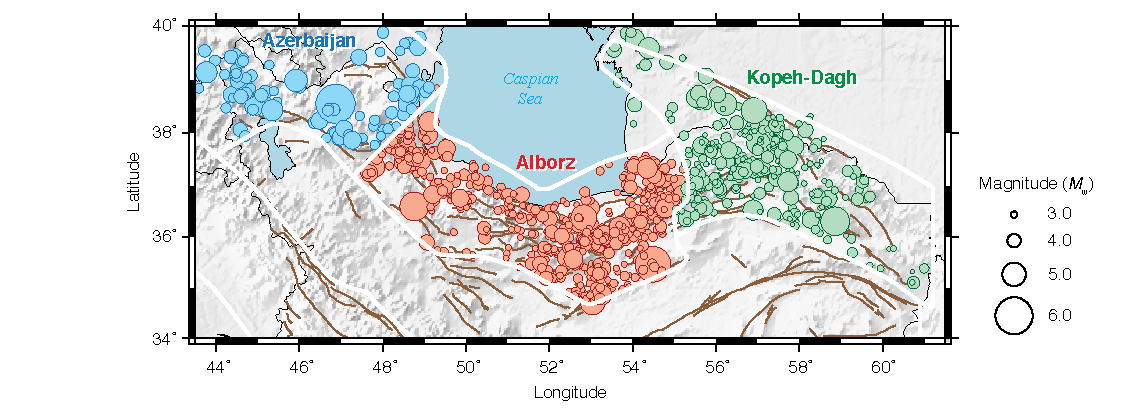
\includegraphics[width=\textwidth]{figures/pdf/figure-03} 
	\caption{Declustered instrumental seismicity of northern Iran for the 2005--2015 period, considering only the events in the seismic zones of interest, namely Azerbaila, Alborz, and Kopeh-Dagh. The size of symbols are proportional to the magnitude of the events, as indicated by the artificial scale shown on the right.}
	\label{fig:seismicity}
\end{figure*}






% \section{Tectonic seismic regions and seismicity parameters}

% \begin{figure*}[t]
% \centering
% 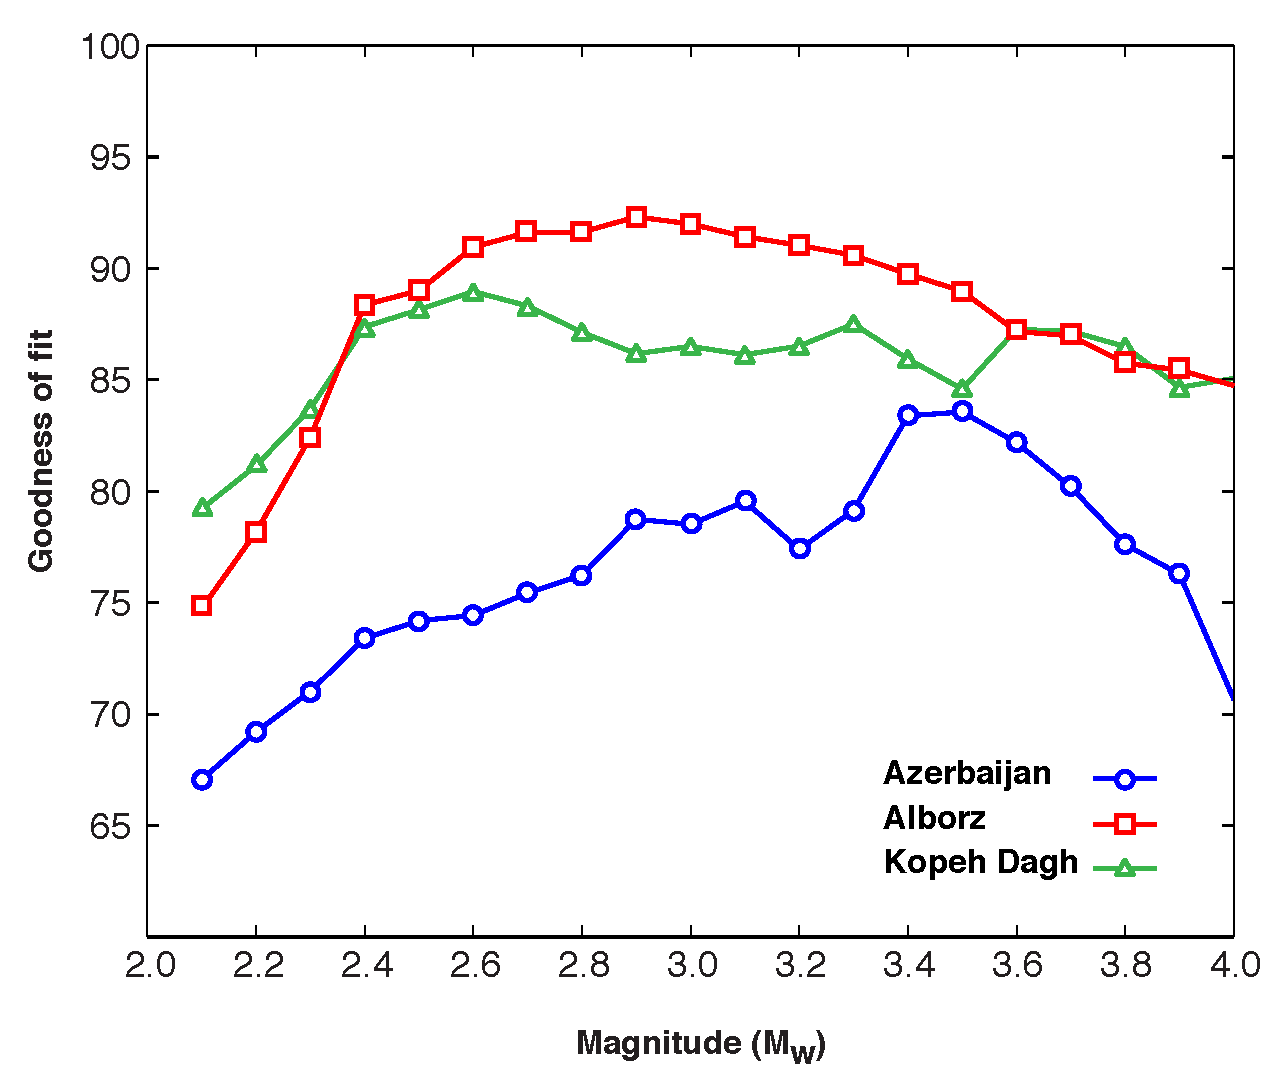
\includegraphics[scale=1]{figures/pdf/Figure03.pdf} 
% \caption{Main fault line and fault system in the region of interest. The borderlines of the seismic zones shown in Fig.~\ref{fig:study_region} are shown in background in gray.}
% \label{fig:faults}
% \end{figure*}

% \subsection{Magnitude Conversion}

% The catalog of recorded earthquakes from 2005-15, downloaded from IIEES, reported earthquakes based on different magnitude scales \citep{IIEES}. The  $M_L$,  $M_S$, and  $mb$  magnitudes were converted through conversion relationships, as defined in  \citet{Zare2014}. Some data were also recorded in  $M_D$  (duration magnitude). These data are reported by the International Seismological Centre (ISC).   \citet{Deniz2010}  developed a set of empirical equations to convert earthquake magnitudes from  $mb$,  $M_D$,  $M_L$, and  $M_S$  scales to  $M_W$  scale using the orthogonal regression procedure. They used data from different data centers, including the ISC, of earthquakes that occurred in Turkey. In this study, we use the conversion equation of  \citet{Deniz2010}  to convert  $M_D$  to  $M_W$. 

% \subsection{Declustering} 

% It is generally assumed that the seismicity of each tectonic seismic source follows a Poissonian occurrence process. Therefore, in order to accomplish this, we decluster the earthquake catalog. In compiling the catalog of events, foreshocks and aftershocks are removed using a declustering methodology  presented by \citet{Gardner1974}. Fig.~\ref{fig:seismicity}  shows the epicenter of declustered instrumental  earthquakes.

% \begin{figure*}[t]
% \centering
% 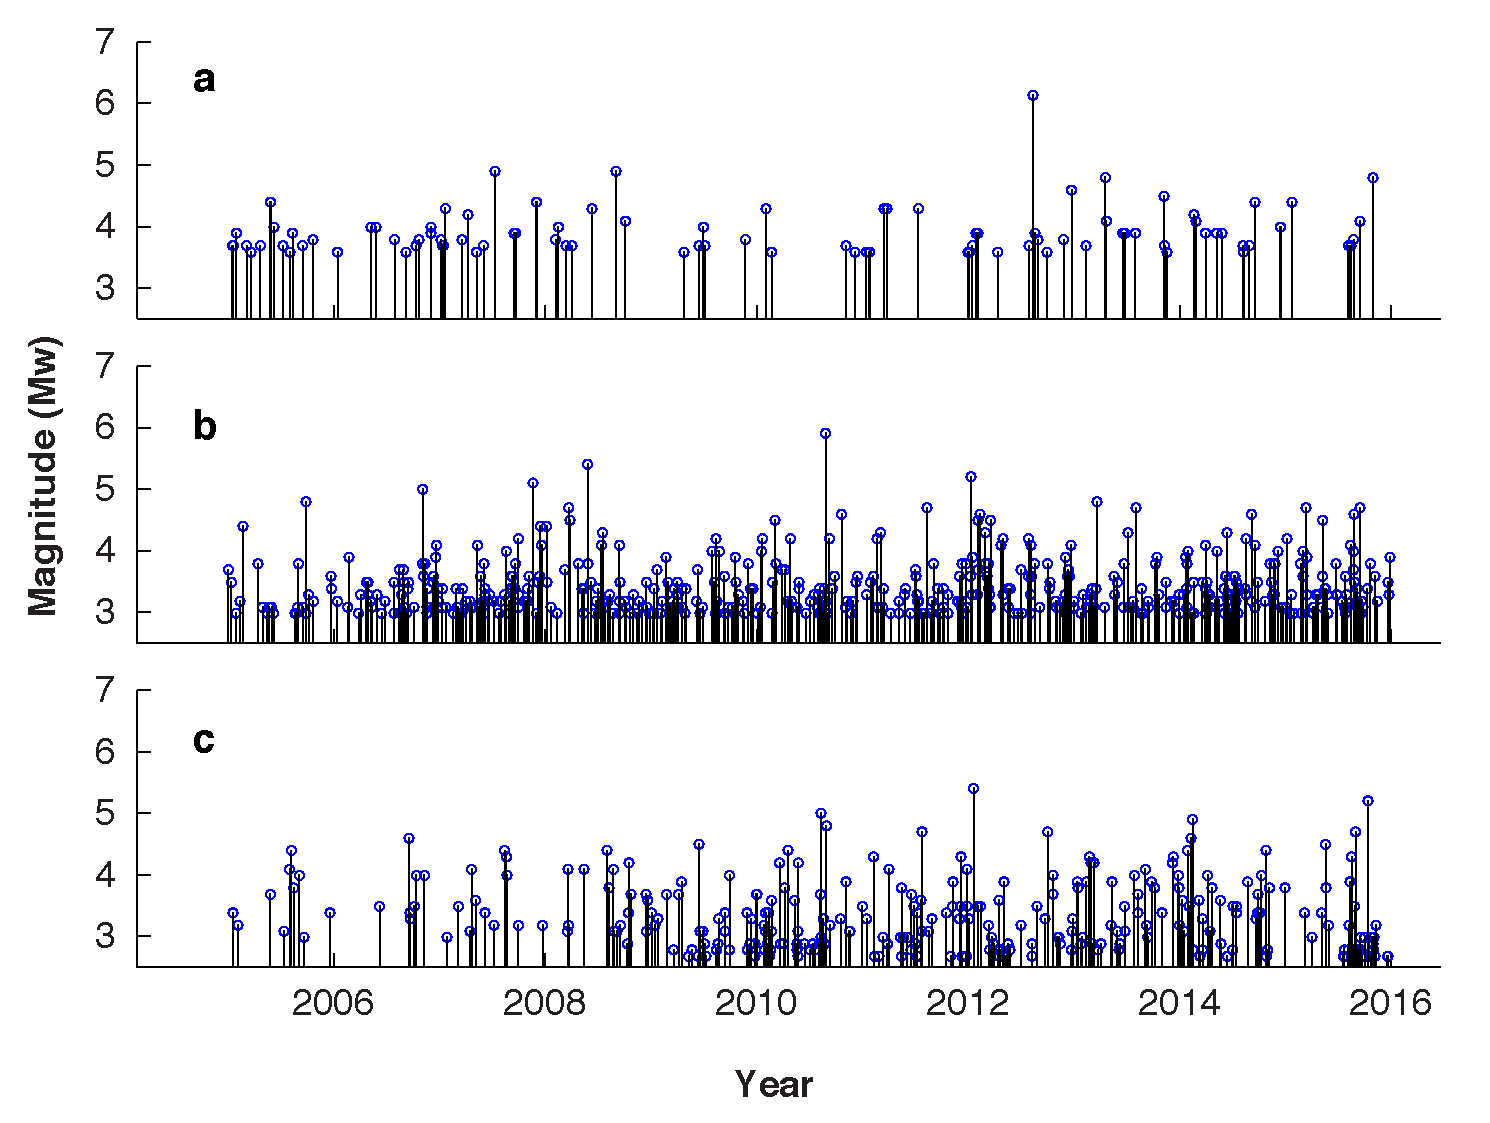
\includegraphics[scale=1]{figures/pdf/Figure04.pdf} 
% \caption{Declustered instrumental seismicity map (2005 - 2015) of northern Iran. Different colors indicate the seismicity of different regions. Size of symbols are proportional to the magnitude of the events.}
% \label{fig:seismicity}
% \end{figure*}
 
% \subsection{Catalog Completeness}

% Catalog completeness is an important factor in studying an earthquake sequence. This characteristic measured as the minimum magnitude of complete recording for earthquake catalog. The completeness magnitude $(M_c)$ is often determined using simple numerical analysis. Two common approaches are maximum curvature method (MAXC) and goodness-of-fit test (GFT)(see \citet{Wiemer2000}). We use the Goodness-of-fit test and compute $M_c$ for each region's catalog. According to the GFT method, a complete catalog should follow the Gutenberg-Richter power law distribution of magnitude. The steps for selecting the completeness magnitude for each catalog include: 1) calculating the a-  and  b-  value based on minimum magnitude; 2) generating  synthetic events based on the achieved value when the cumulative number of events obey the power law distribution; and 3) calculating goodness of fit for predicted and observed cumulative numbers for each magnitude bin  \citep{Wiemer2000}. We increase the minimum magnitude and repeat the process in order to calculate the goodness of fit for each magnitude.  \citet{Wiemer2000} assumed a goodness of fit of 90\% as a threshold to select the completeness of the catalog. However,  not all frequency-magnitude distributions reach the 90\% mark. Fig.~\ref{fig:completeness} shows the goodness-of-fit values for three tectonic seismic regions. For each tectonic seismic region, we select the magnitude corresponding to the highest goodness of fit or the first magnitude with the goodness of fit greater than 90\%.

% \begin{figure}[t]
% \centering
% 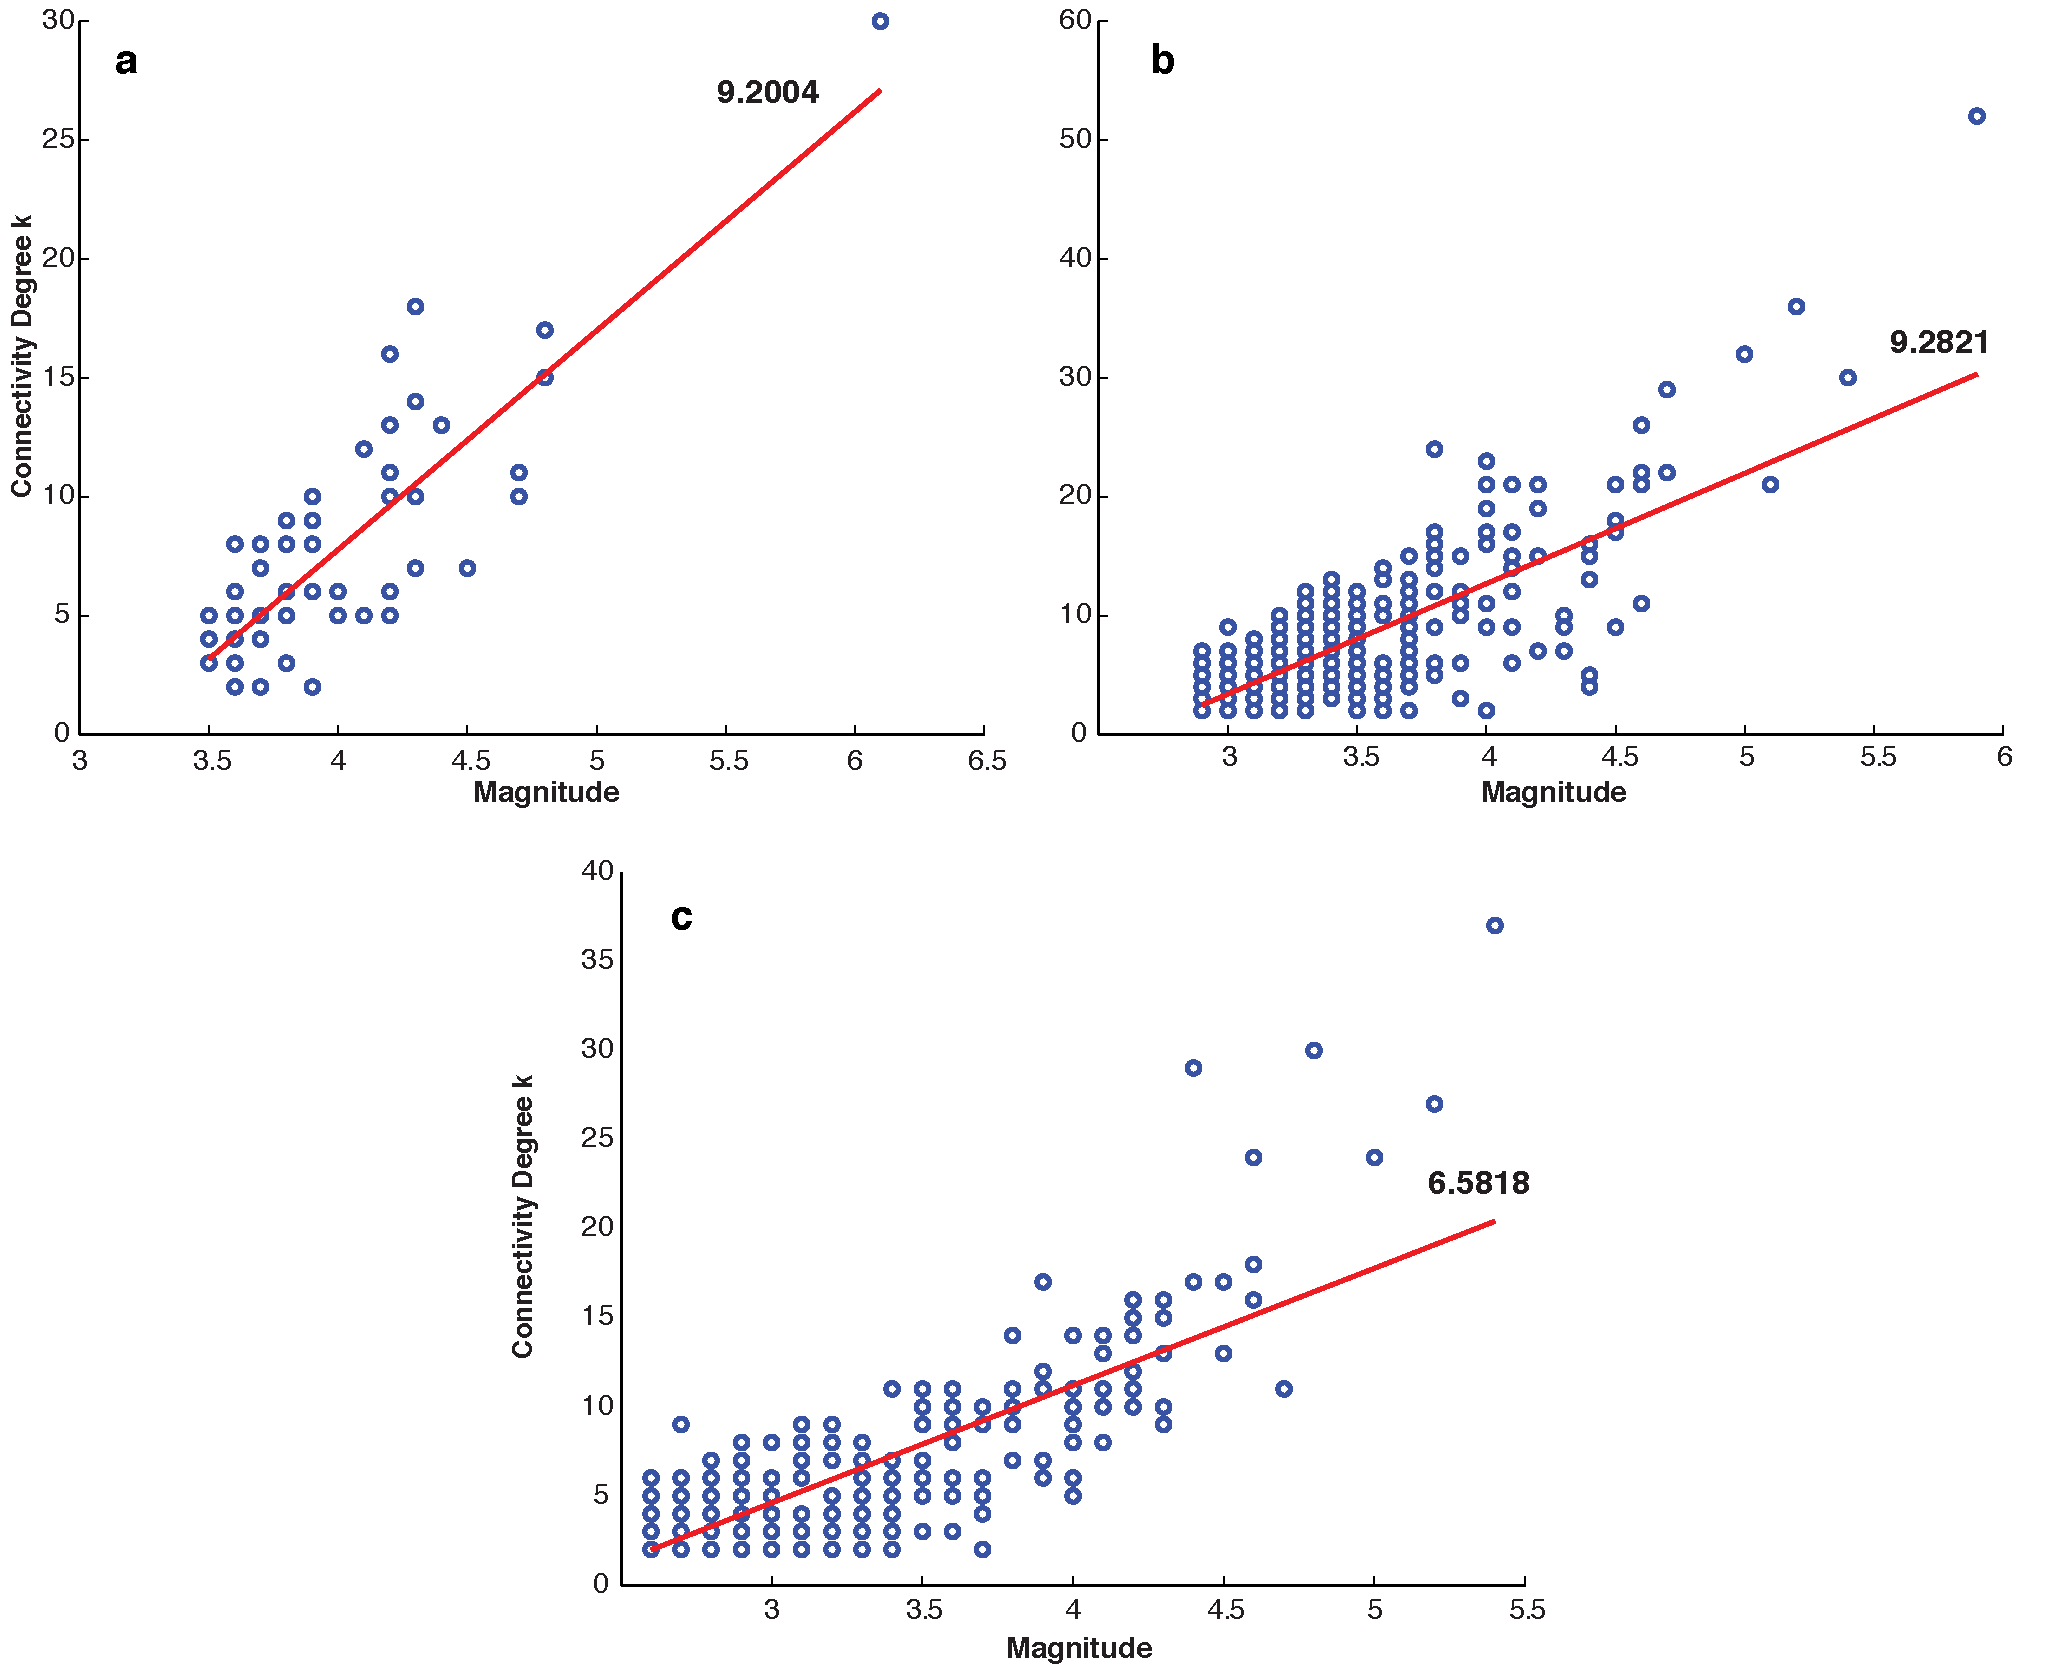
\includegraphics[width=0.45\textwidth]{figures/pdf/Figure05.pdf} 
% \caption{ Selection of completeness magnitude $M_c$ of the three tectonic seismic regions in northern Iran in 2005-15 period. The symbols indicate the computed GFT values as function of the earthquake magnitude. The horizontal dashed line indicates the desired threshold for the goodness of fit value at 90 percent. The vertical dashed lines indicate the completeness magnitude of each tectonic seismic region.}
% \label{fig:completeness}
% \end{figure} 

% Based on the results represented in Fig.~\ref{fig:completeness}, we select the minimum magnitudes for complete recording,  $M_c$ , is 3.5, 2.6, and 2.6 for Azerbaijan, Alborz, and Kopeh Dagh, respectively. Fig.~\ref{fig:mag-time}  shows the magnitude time series of the declustered data for the three regions. Earthquakes with magnitude greater than the completeness magnitude are represented. 

% \begin{figure*}[t]
% 	\centering
% 	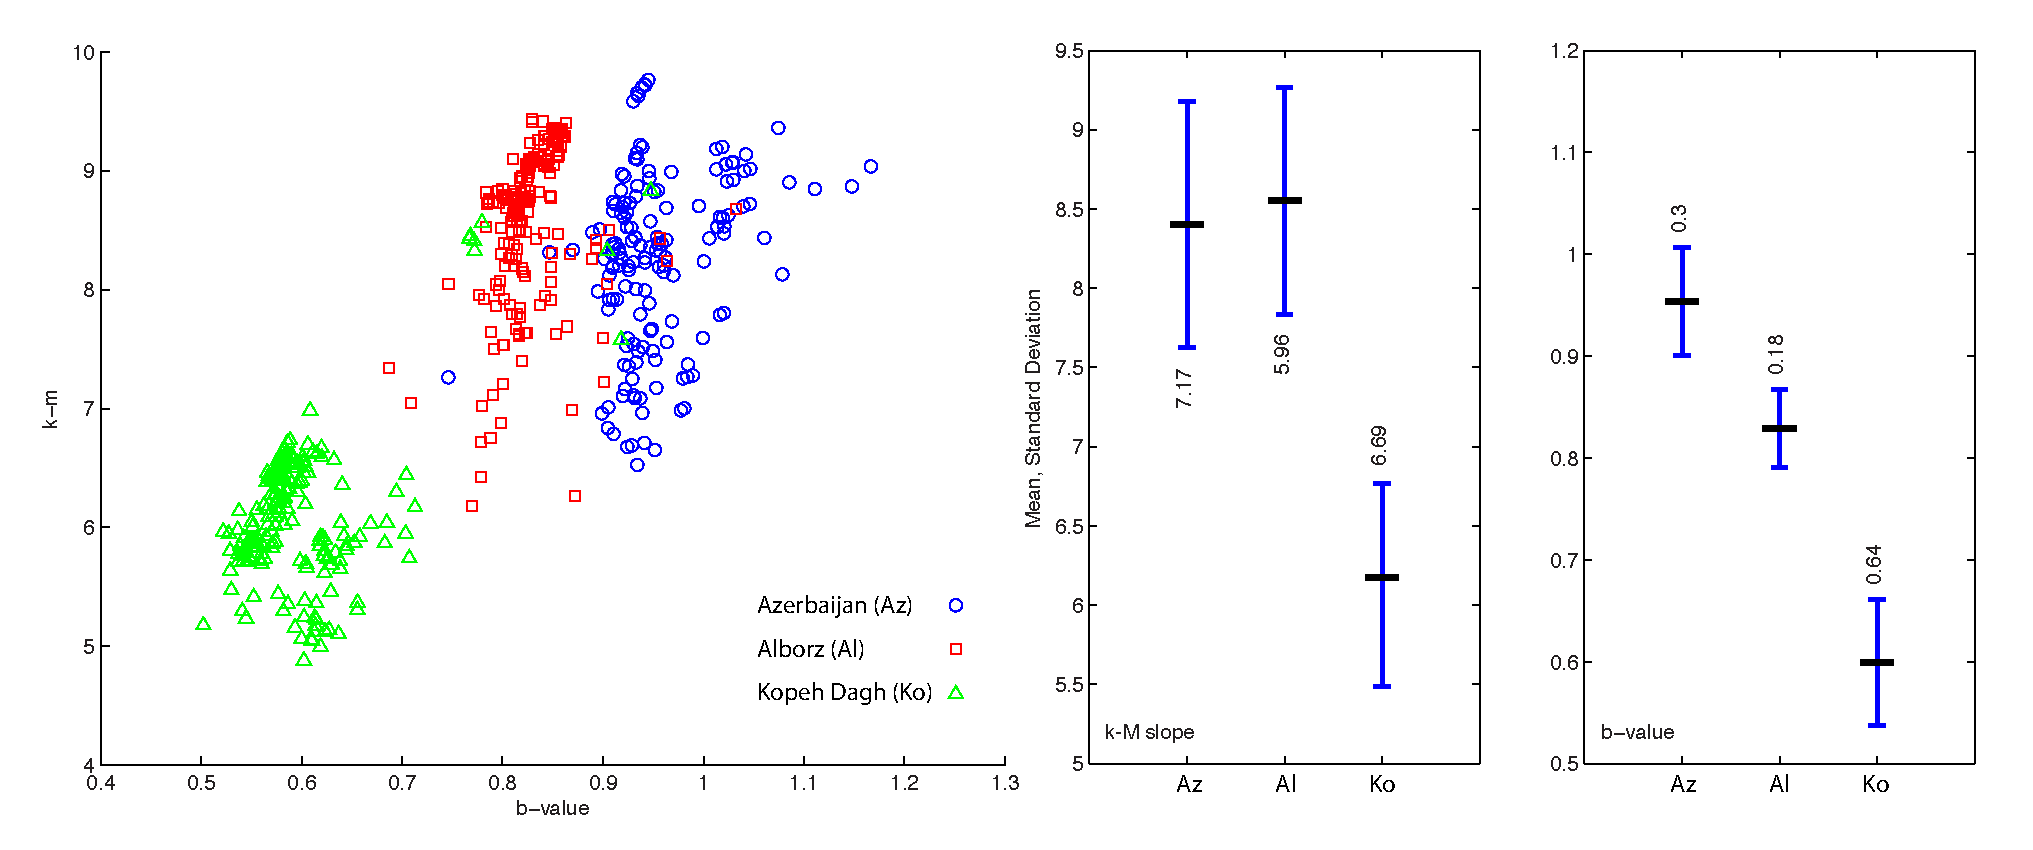
\includegraphics[scale=0.8]{figures/pdf/Figure06.pdf} 
% 	\caption{Variation of moment magnitude ($M_w$) of 2005-2015 earthquake for north Iran as a function of time. The figure only represents the declustered events greater than minimum magnitude. The 2012 $M_w 6.4$ East Azerbaijan, 2010 $M_w 5.8$ Damghan, and 2012 $M_w 5.4$ Neyshabur earthquakes are clearly visible as maximum values in Azerbaijan (Az),  Alborz (Az), and Kopeh Dagh (Ko) magnitude-time series.}
% 	\label{fig:mag-time}
% \end{figure*}

